%%%%%%%%%%%%%%%%%%%%%%%%%%%%%%%%%%%%%%%%%%%%%%%%%%%%%%%%%%%%%%%%%%%%
\section{Integration and Installation}
\label{sec:fdsp-apa-install}

Completed \dwords{apa} will be shipped from the \dword{apa} production sites to an Integration Facility (IF) for integration with the TPC \dword{fe} electronics and \dwords{pd}.  The IF location is not decided, but facilities near the Sanford site are being considered.   Activities at the IF will include extensive \dword{qc} testing to ensure the functioning of the fully integrated \dwords{apa}.  Once checked, the \dwords{apa} are repackaged for final transport to SURF. Each \dword{apa}, still in its transport crate, will be hung from the Ross Shaft cage by a sling and transported underground where it will be stored in a waiting area.  Pairs of \dwords{apa} must be linked in their vertical configuration and cables ran from both the lower and upper \dwords{apa} in an area just outside the cryostat.  Once completed, the pair enters through the \dword{tco} onto the \dword{dss} and is moved into its final position.  Final checkout tests will be performed once the \dwords{apa} are in place.

The integration with the \dwords{pd} is expected to be done at the Integration Facility. However, there is an alternative plan where they would be installed at the \dword{apa} production sites (the specifics of the plan needs to be developed with the \dword{pds} consortium and depend on the final \dword{pds} design). The TPC \dword{fe} electronics will be installed  at the IF and the exact installation sequence will be developed with the electronics consortium.

A conceptual layout of the space required at the Integration Facility is being developed. An overhead crane is needed to lift \dwords{apa} out of their shipping crate and maneuver them through the facility.  Most of the handling areas will need to be embedded in a class \num{100000} clean tent. Finally, a cold box will be available for \dword{qc} testing of the electronics once installed on the \dword{apa} (see Section~\ref{sec:fdsp-apa-install-qc_if}).  

%\begin{dunefigure}[Schematics of the layout of the IF testing area]{fig:testlayout}{A schematic of the layout for the testing area at the IF. Most of this area has to be embedded in a clean environment (i.e. tent).}
%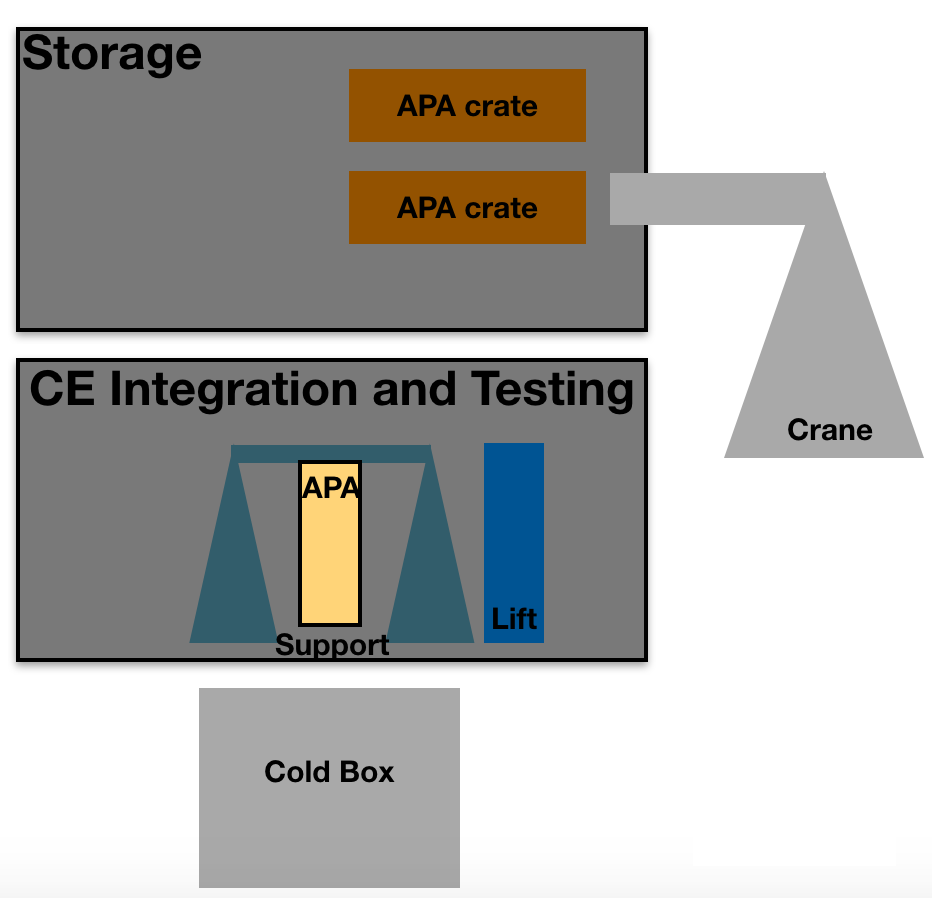
\includegraphics[width=0.4\textwidth]{test_layout.png} 
%\end{dunefigure}


%%%%%%%%%%%%%%%%%%%%%%%%%%%%%%%%%%%%%%%%%%%%%%%%%%%%%%%%%%%%%%%%%%%%
\subsection{Transport and Handling}
\label{sec:fdsp-apa-install-transport}

Custom designed crates will be used for transport between the production sites and the IF, and between the IF and SURF. The design of the crates is still being finalized, but there are currently two possible approaches. The first is to use less expensive, disposable crates for transport to the IF and fewer, more expensive crates for transport underground, which are reused between the IF and underground. The second option is a single crate that is used for all transport stages. The transport underground requires a design that will allow a 180$^{\circ}$ rotation of the crate. 

%\begin{dunefigure}[Draft of the \dword{apa} transport crates]{fig:crate}{A schematic design of the \dword{apa} transport crate (note that the material will not be wood).}
%\includegraphics[width=0.5\textwidth]{tp3-5-1-fig1.jpg} 
%\end{dunefigure}

The handling of the \dwords{apa} at the IF and underground is done with overhead cranes. Once the \dwords{apa} are repackaged in the crates, they  will be loaded on a truck, driven to the mine, transported to the cage, secured on the sling under the cage (see figure \ref{fig:cagetransport}), lowered down and moved to the underground storage area.

\begin{dunefigure}[\dword{apa} suspended beneath the mine shaft cage]{fig:cagetransport}{The \dword{apa} crate (in blue) will be brought underground with a sling under the elevator cage (the green box at the top of the figure). The insertion into the crate at the surface is done from the back of the cage, but the extraction underground must be done from the front of the cage. The \dword{apa} crate must, therefore, be able to be rotated  by 180$^\circ$ in the sling.}
\setlength{\fboxsep}{0pt}
\setlength{\fboxrule}{0.5pt}
%\fbox{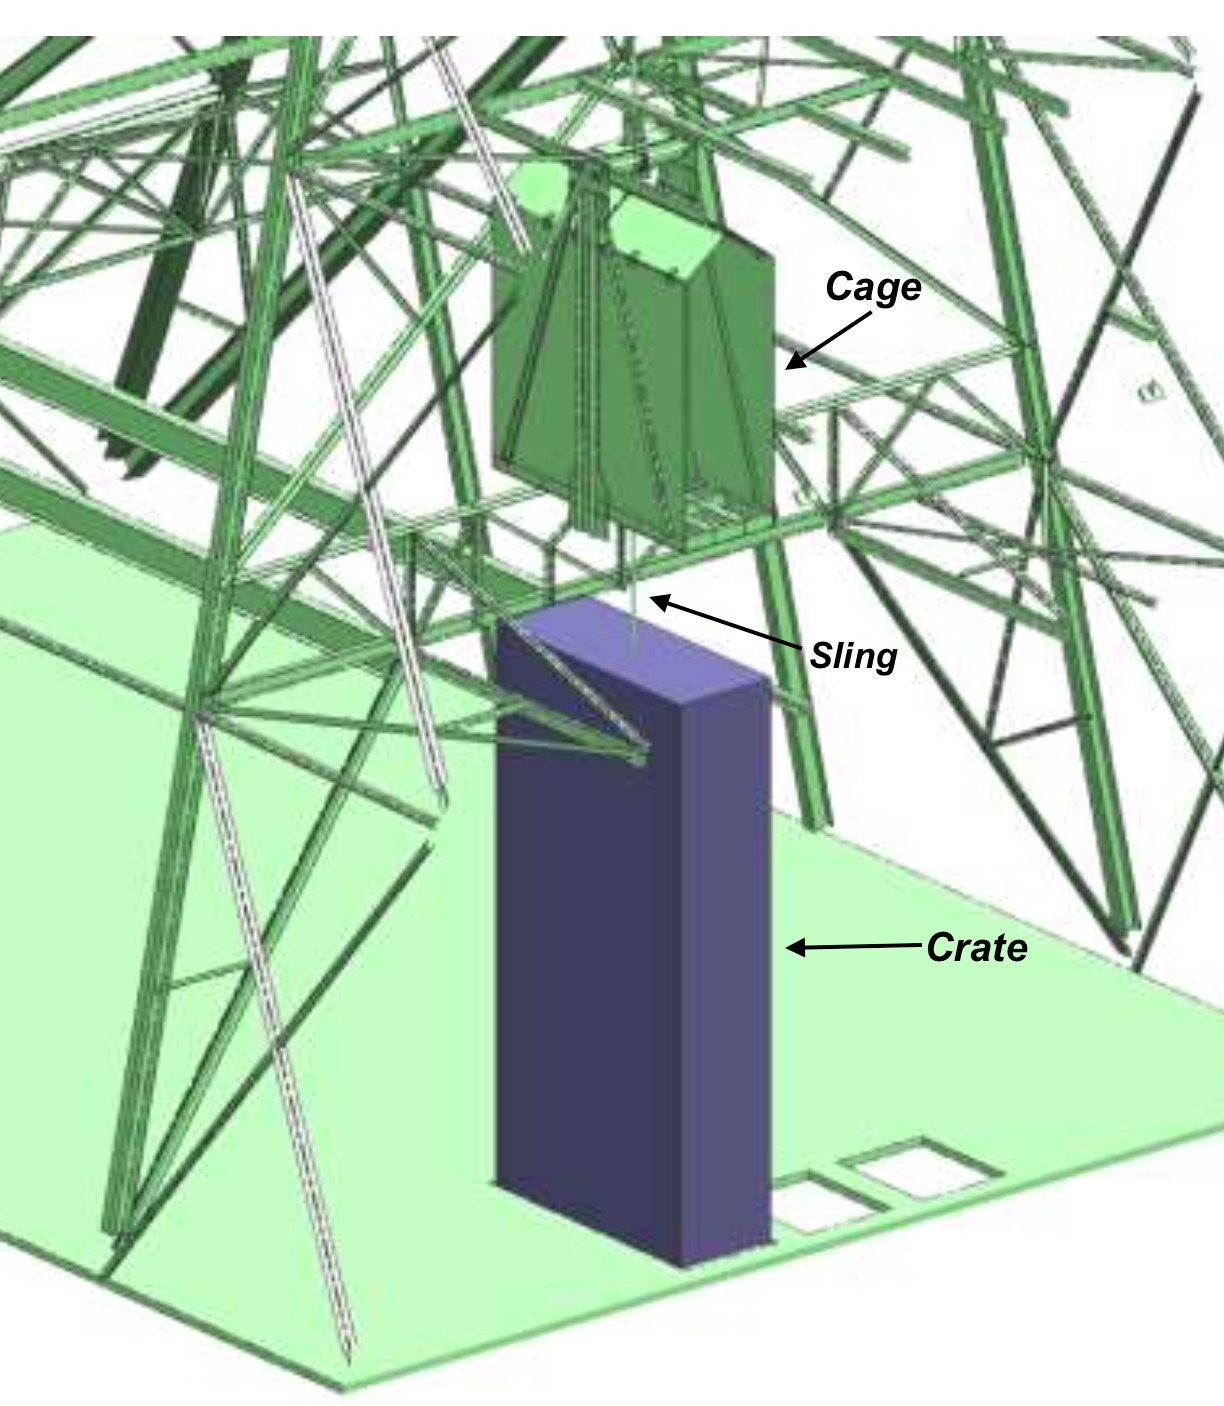
\includegraphics[width=0.4\textwidth, trim=0mm 20mm 0mm 20mm,clip]{apa-cage.jpg}} 
\end{dunefigure}


%%%%%%%%%%%%%%%%%%%%%%%%%%%%%%%%%%%%%%%%%%%%%%%%%%%%%%%%%%%%%%%%%%%%
\subsection{\dword{apa}-to-\dword{apa} Assembly and Installation in the Cryostat}
\label{sec:fdsp-apa-install-cryostat}

Once underground, there will be a small storage area for stockpiling \dwords{apa} (see Figure~\ref{fig:handling}). When ready for installation, each \dword{apa} is extracted from its crate, inspected and rotated to be lowered into the area just outside of the \dword{tco} in the cryostat. Two \dwords{apa} are lowered in front of the \dword{tco} where they are linked and cabled. The details of the cabling are still being finalized, but the main option is currently to pass all the cables inside the \dword{apa} frame tubes (see Section~\ref{sec:fdsp-apa-intfc-apa}).

%\begin{dunefigure}[\dword{apa} cabling]{fig:\dword{apa}cables}{Proposed cabling solution for the \dwords{apa}. }
%\begin{tabular}{cc}
%\includegraphics[width=0.5\textwidth]{\dword{apa}_cables_2.png} 
%\includegraphics[width=0.4\textwidth]{\dword{apa}_cables.jpeg} 
%\end{tabular}
%\end{dunefigure}

%\begin{dunefigure}[\dwords{apa} in the \dword{tco}]{fig:\dword{apa}_\dword{tco}}{Left: Top and bottom \dwords{apa} placed in the \dword{tco} for cabling and linking. Center: Linking bracket current design. Right: Current \dword{apa} linking solution.}
%\begin{tabular}{cc}
%\includegraphics[width=0.3\textwidth]{\dword{apa}_link.png} 
%\includegraphics[width=0.4\textwidth]{\dword{apa}_link_2.png} 
%\end{tabular}
%\end{dunefigure}

Finally, when the two \dwords{apa} are fully cabled, they are placed onto the DSS inside the cryostat (see bottom right of Figure~\ref{fig:handling}) and moved to their location in the cryostat where final integration tests will be performed.  For more information on the detector support structure and installation into the cryostat, see %the Technical Coordination 
Chapter~\ref{ch:fdsp-coord}. 

\begin{dunefigure}[Underground handling of the \dwords{apa}]{fig:handling}{(Top row) Handling of an \dword{apa} in the underground storage area where the \dwords{apa} are extracted from the crates, inspected, and readied for installation in the cryostat. (Bottom row) A pair of \dwords{apa} are brought into the space just outside the \dword{tco} to be linked and cabled, then connected to the \dword{dss} and moved into their final position inside the cryostat.}
\setlength{\fboxsep}{0pt}
\setlength{\fboxrule}{0.5pt}
\centering
%\fbox{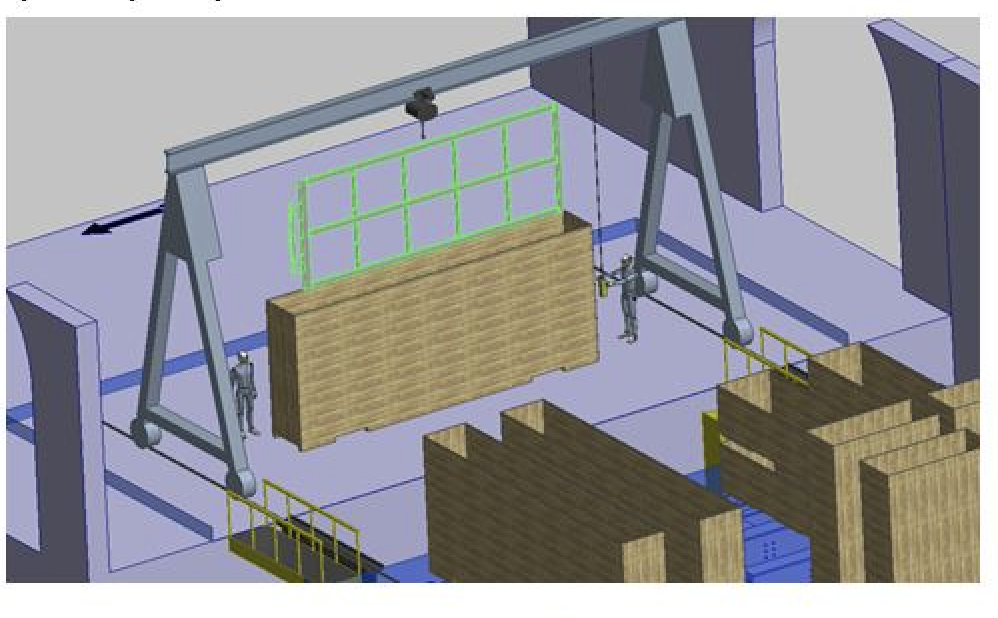
\includegraphics[height=0.195\textheight,trim=8mm 8mm 20mm 4mm,clip]{apa-install-1.png}} 
%\fbox{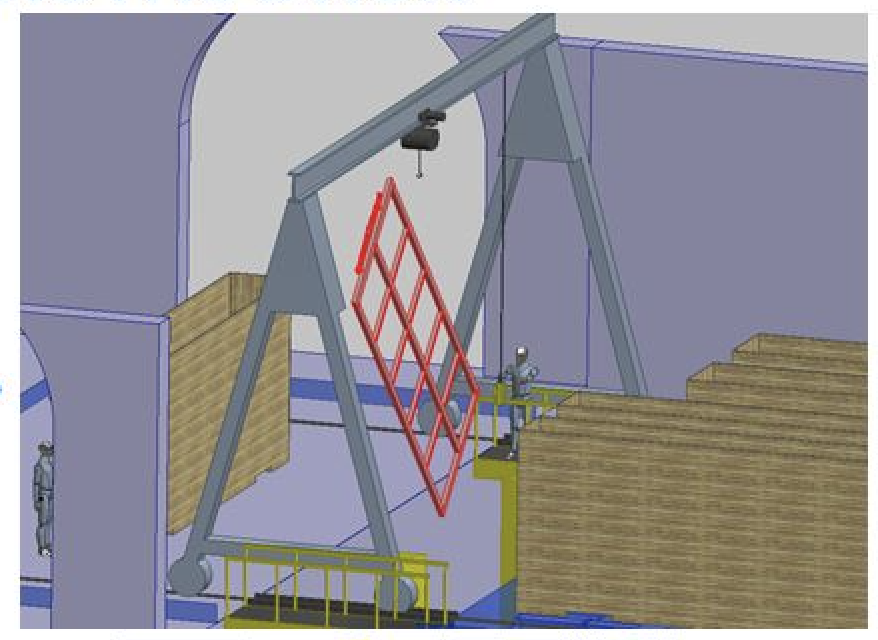
\includegraphics[height=0.195\textheight,trim=8mm 4mm 20mm 4mm,clip]{apa-install-2.png}} 
%\fbox{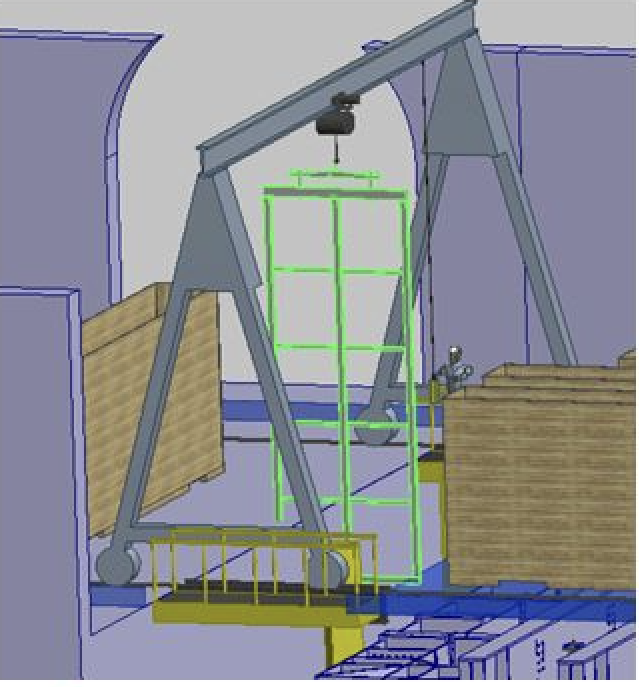
\includegraphics[height=0.195\textheight,trim=4mm 4mm 4mm 4mm,clip]{apa-install-3.png}} 
%\\ \vspace*{1.5mm}
\hspace*{-.25mm}
%\fbox{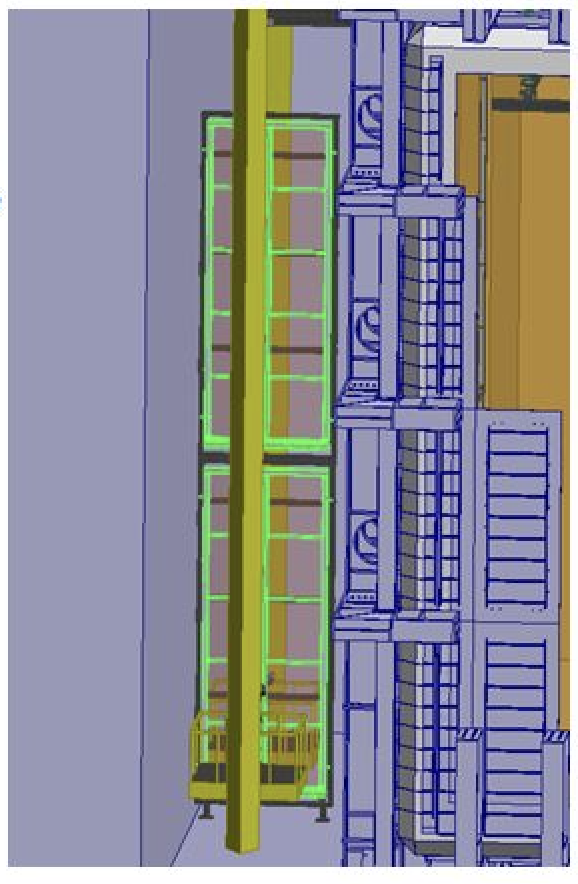
\includegraphics[height=0.37\textheight,trim=4mm 4mm 4mm 4mm,clip]{apa-install-4.png}}
\hspace*{1.mm}
%\fbox{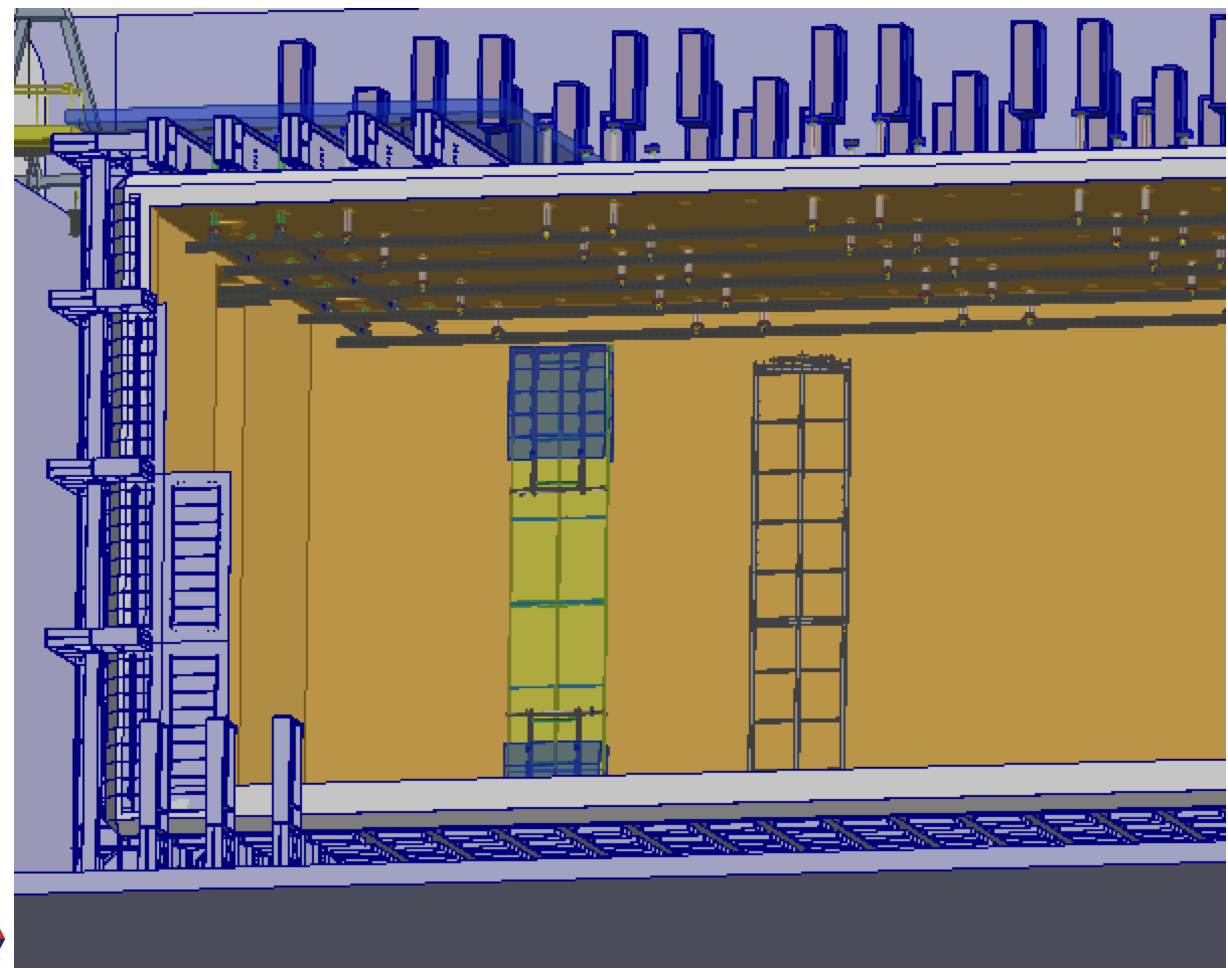
\includegraphics[height=0.37\textheight,trim=4mm 4mm 4mm 4mm,clip]{apa-install-5.png}}
\end{dunefigure}
%\begin{dunefigure}[\dwords{apa} in the cryostat]{fig:\dword{apa}_cryostat}{Top/bottom \dword{apa} pairs are moved inside the cryostat to their final location.}
%\includegraphics[width=0.5\textwidth]{\dword{apa}_cryostat.png} 
%\end{dunefigure}


%%%%%%%%%%%%%%%%%%%%%%%%%%%%%%%%%%%%%%%%%%%%%%%%%%%%%%%%%%%%%%%%%%%%
\subsection{Quality Assurance and Quality Control in Integration and Installation}
\label{sec:fdsp-apa-install-calib}

The \dword{qc} related to integration and installation has two main testing campaigns, one at the Integration Facility (IF) and one once the \dwords{apa} are installed into their location in the cryostat. Some details are still under development by the installation and integration team within the \dword{apa} consortium. 

A dedicated database for \dword{qc} is required to keep track of all the components for all the \dwords{apa} at the different stages of the integration and installation. A simple and practical method of tagging critical parts in the \dword{apa} is also under development for efficient integration.

The \dword{qa} related to integration and installation is heavily based on the \dword{pdsp} experience and at this point no dedicated \dword{qa} protocol is developed. The full development will be done by the installation and integration team in the \dword{apa} consortium. 

%%%%%%%%%%%%%%%%%%%%%
\subsubsection{Quality Control at the Integration Facility}
\label{sec:fdsp-apa-install-qc_if}

All the active detector components will be shipped to the IF for integration and for testing. It is at that location that we will have the most time to perform tests and this step will be critical for ensuring high performance of the integrated \dwords{apa}. The exact time scale of \dword{apa} testing needs to be finalized based on information from the production sites and on the installation schedule. 


%Table \ref{tab:qclist} shows a summary of the quality control tests that will be performed at the IF. The details of each is given below. %Figure \ref{fig:testlayout} shows an example of the layout of the testing area at the IF.

\begin{comment}
\begin{dunetable}[QC List]{l|c|c}{tab:qclist}{List of tests performed for Quality Control upon reception at the integration facility}   
Test to perform   &  Number of wires/channels & Acceptable values, action\\ 
Visual inspection & All & > 99\% intact \\
Wire tension      & 10$\%$ sample & 5 $\pm$ \SI{1}{N}\\
Wire continuity   & All & $-$\\
Current leakage   & All & < X $\mu$A \\
Electronics connections & All & Perfect (> 99$\%$)\\
%Noise             & All &  $\pm$ XX (> 99$\%$)\\
Cold test         & All & All intact (> 99$\%$)\\
\textbf{Overall}  & \textbf{All} & \textbf{At least 99$\%$ fully operational}\\
\end{dunetable}
\end{comment}

After unpacking an \dword{apa} at the IF, a thorough visual inspection will be performed. Tension measurements will be made for a sample of around \num{350} wires (representing $\sim$10\% of the wires). The default technique is the laser method that has been used for \dword{pdsp}.  The method works well, but is time consuming, so alternative methods that use voltage measurements are also being pursued to reduce the measuring time. Such improved methods could allow a larger number of wires (even the full \dword{apa}) to be measured. 

Tension values will be recorded in the database and compared with the original tension measurements performed at the production sites. Definite guidance for the acceptable tension values will be available to inform decisions on the quality of the \dword{apa}. Clear pass/fail criteria % I think slash ok in this construction; leaving it in (anne)
will be provided as well as clear procedures to deal with individual wires laying outside the acceptable values. %Exact relation between lower or higher tension and the acceptance of a channel still needs to be worked out. 
This guidance will be based on the \dword{pdsp} experience, where the tension of some wires have changed during the production to installation process. In addition, a continuity test and a leakage current test will be performed on all the wires and the data will also be recorded in the database. 

Once the electronics are installed by the electronics consortium, dedicated testing of the \dword{apa} readout will be performed. The integrated \dword{apa} should be inserted in the cold box and the electronics performance can be tested adequately. A strict guidance will be available to assess the pass/fail criteria for each \dword{apa} during these tests. Here too, guidance from \dword{pdsp} and development tests will guide the exact criteria. Close collaboration with the electronics consortium will be necessary.

When all the tests have been successfully performed and more than \num{99}\,\% of the channels are confirmed functional, the \dword{apa} will be tagged as good and prepared for shipping to SURF.

%%%%%%%%%%%%%%%%%%%%%%%%%%
\subsubsection{Quality Control Underground}
\label{sec:fdsp-apa-install-qc_underground}

There are three opportunities to test the \dwords{apa} underground: in the storage area, once secured in front of the \dword{tco}, or once positioned at their final location in the cryostat. The latter is the most important and it might be good to save time to perform the final tests once the full \textit{APA-CPA-APA-CPA-APA wall} is installed (\dwords{cpa} are described in Chapter~\ref{ch:fdsp-hv}). This brings the risk that if serious problems are found, \dwords{apa} are harder (more time-consuming) to move out.

%\paragraph{Tests underground in the storage/unpacking area}
The \dwords{apa} will be unpacked in the storage area underground (see Figure~\ref{fig:storage}). Space in this area is very limited and only visual inspection will be performed during unpacking. If clear defects are visible, the \dword{apa} will be returned to the IF for further investigation.

\begin{dunefigure}[Schematics of the underground storage area; full A-C-A-C-A wall in the cryostat]{fig:storage}{Left: A schematic of the layout for the storage and unpacking area underground. Right: A schematic of the layout of a full APA-CPA-APA-CPA-APA wall installed in the cryostat.}
\setlength{\fboxsep}{0pt}
\setlength{\fboxrule}{0.5pt}
%\fbox{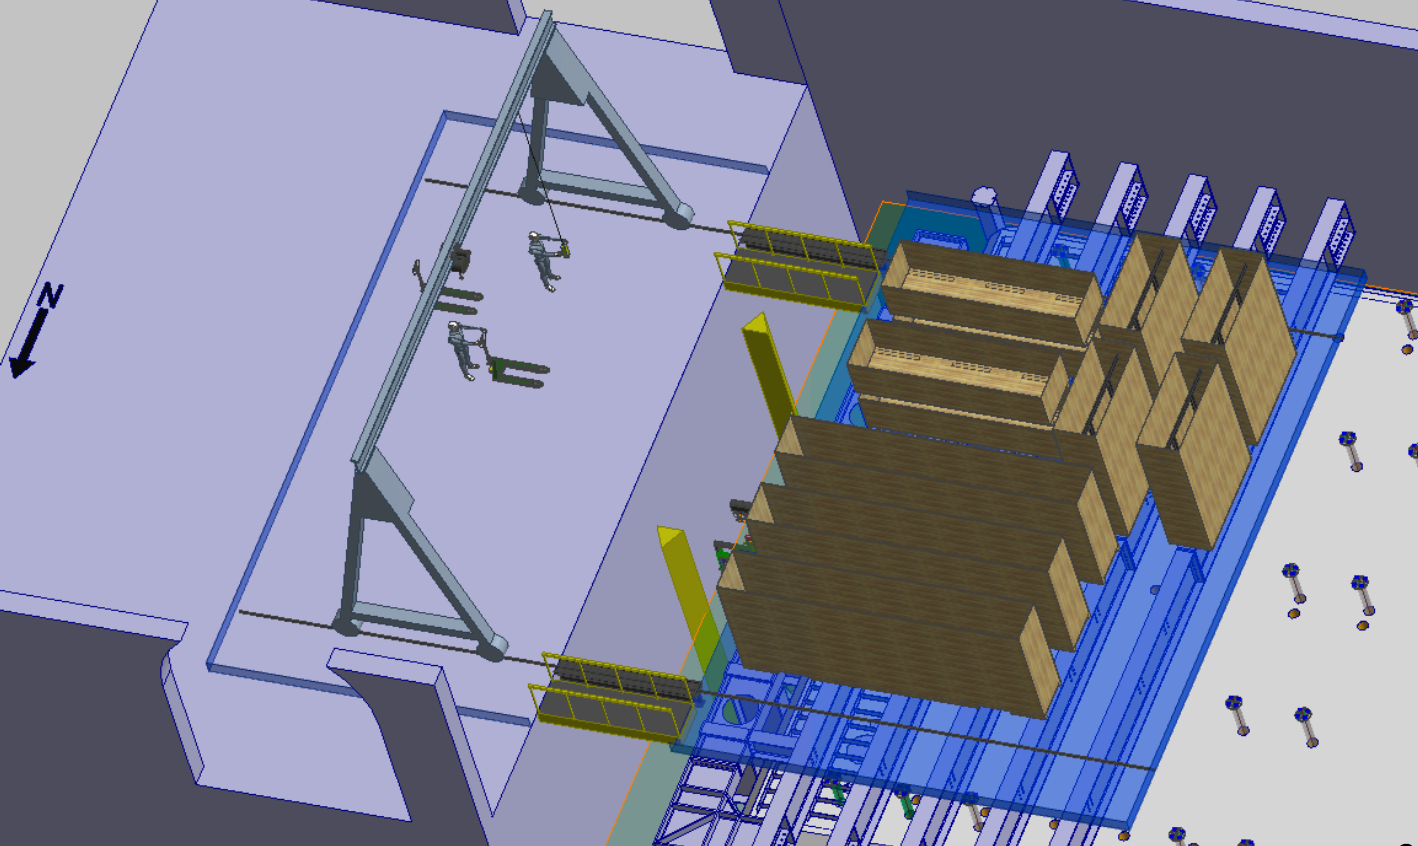
\includegraphics[height=0.26\textheight]{apa-underground-storage.png}} 
%\fbox{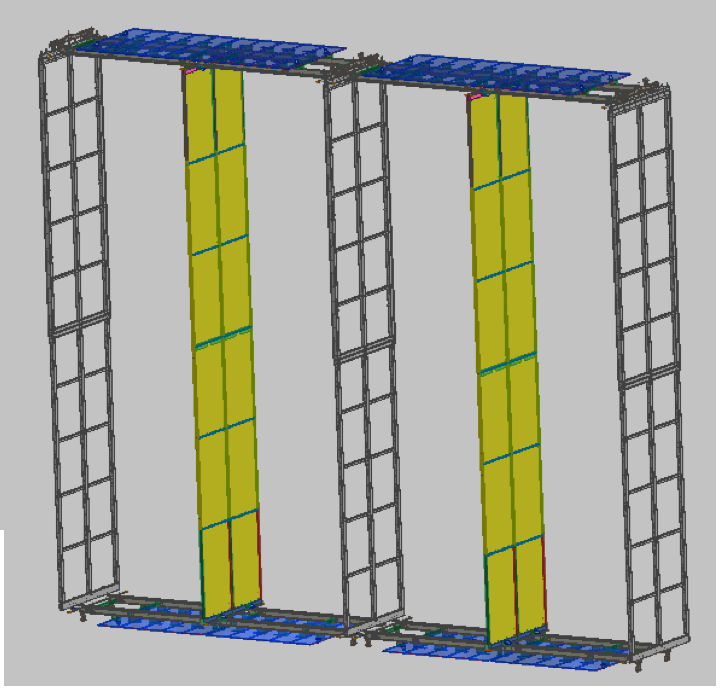
\includegraphics[height=0.26\textheight,trim=0mm 2mm 2mm 0mm,clip]{apa-acaca-wall.png}}
\end{dunefigure}

%\paragraph{Tests underground in the \dword{tco} area}
Pairs of \dwords{apa} (top and bottom) will be lowered in front of the \dword{tco} to be linked and cabled. Once the cabling is finished a connection test will need to be performed to ensure adequate cabling. Due to the very restrictive space near the \dword{tco} (see Figure~\ref{fig:handling}), no additional tests other than visual inspection will be performed at that time and the cabled and linked \dwords{apa} will be positioned in their final location in the cryostat.

%\begin{dunefigure}[Schematics of the \dword{tco}  area]{fig:tco}{A schematic of the layout for the \dword{tco} area underground.}
%\begin{tabular}{cc}
%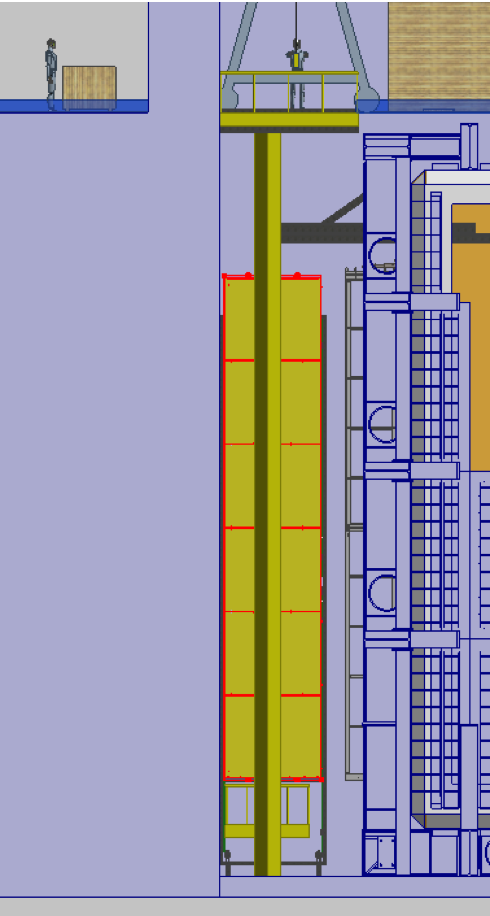
\includegraphics[width=0.23\textwidth]{tco1.png} &
%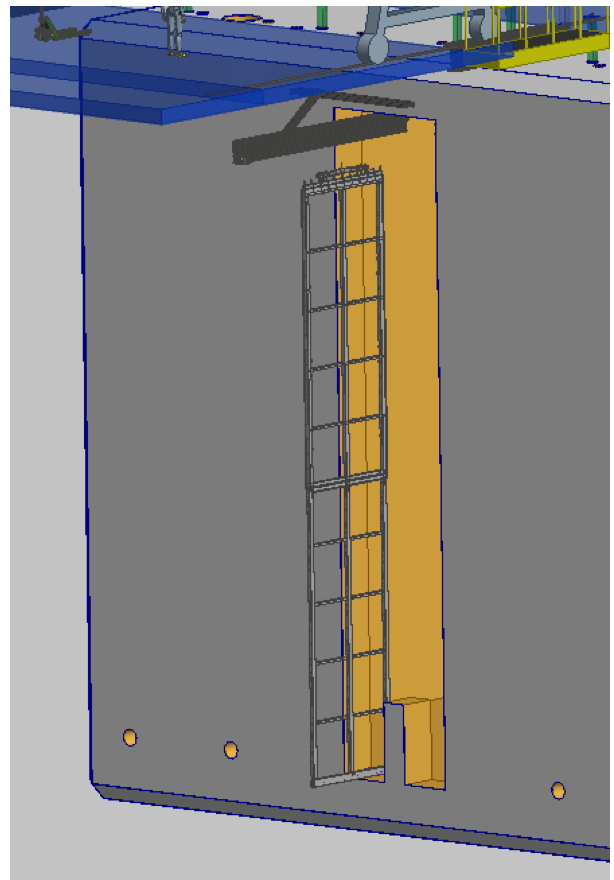
\includegraphics[width=0.3\textwidth]{tco2.png}
%\end{tabular}
%\end{dunefigure}

%\paragraph{Tests underground in the cryostat}
The current goal is to install a full APA-CPA-APA-CPA-APA wall every week (see Figure~\ref{fig:storage}, right). After each wall is installed, the night crew will have time for final testing of the installed \dword{apa}. There are currently two testing models, one where the night crew will test \dword{apa} pairs as they are installed (every two days), and the other model where the night crew will test the full wall at once. The decision between the two models will be made when accurate estimates of the time needed for the testing will be available.

%\begin{dunefigure}[Schematics of the wall in the cryostat]{fig:wall}{A schematic of the layout of a full \dword{apa}-\dword{cpa}-\dword{apa}-\dword{cpa}-\dword{apa} wall installed in the cryostat.}
%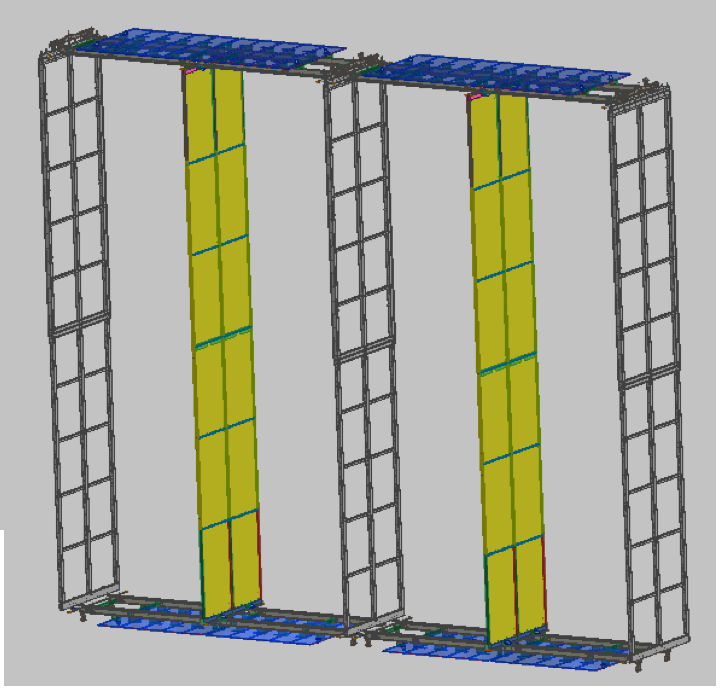
\includegraphics[width=0.4\textwidth]{wall.png}
%\end{dunefigure}

The tests performed will be the same described above at the IF. Tension on a smaller set of wires will be measured ($\sim$5\%, potentially more if a quicker tension method is developed) to ensure that the installation operations did not alter the \dwords{apa}. Since the complete integration is now done, a full readout test can be performed. Short runs will be taken with the \dword{daq} system to ensure that the readout is fully operational. The details of these tests still need to be developed to provide efficient assessment of the integrated \dwords{apa}. If an \dword{apa} appears to have more than \num{1}\,\% of the channels not functioning, the \dword{apa} would need to be sent back to the IF.

\subsubsection{Quality Assurance}

We will rely on the \dword{pdsp} experience to assess most of the \dword{qa} protocols. The dedicated \dword{qa} plan during production should ensure that the \dwords{apa} meet the requirements and the installation steps should not modify them. The control of the quality of each wire along the installation steps will ensure fully functioning \dwords{apa}. The detailed \dword{qa} program is currently under development by the installation and integration group in the \dword{apa} Consortium.


